\section{Performance Validation in Simulation - (Lead by Abhishek, Amelia, Lucian, Vlad)}\label{sec:mc}

The charge collection of the MALTA2 pixel has been derived from testbeam data \cite{MALTA2_CCParameterization}.
A parametric simulation approach is used that has been validated against data \cite{MALTAFastSim_Arxiv}.
A quad module made of four sensors in series simulated in GEANT4. Each sensor is identical but has time difference because of proximity (ref simulated geometry and schemtic). 
Characterization of sensors: Each sensor physical properties. 
fast simulation and Readout implementation(digitization) and tracking with custom configuration. 


\subsection{Telescope geometry and setup in simulation}
\begin{figure}[t]
    \centering
    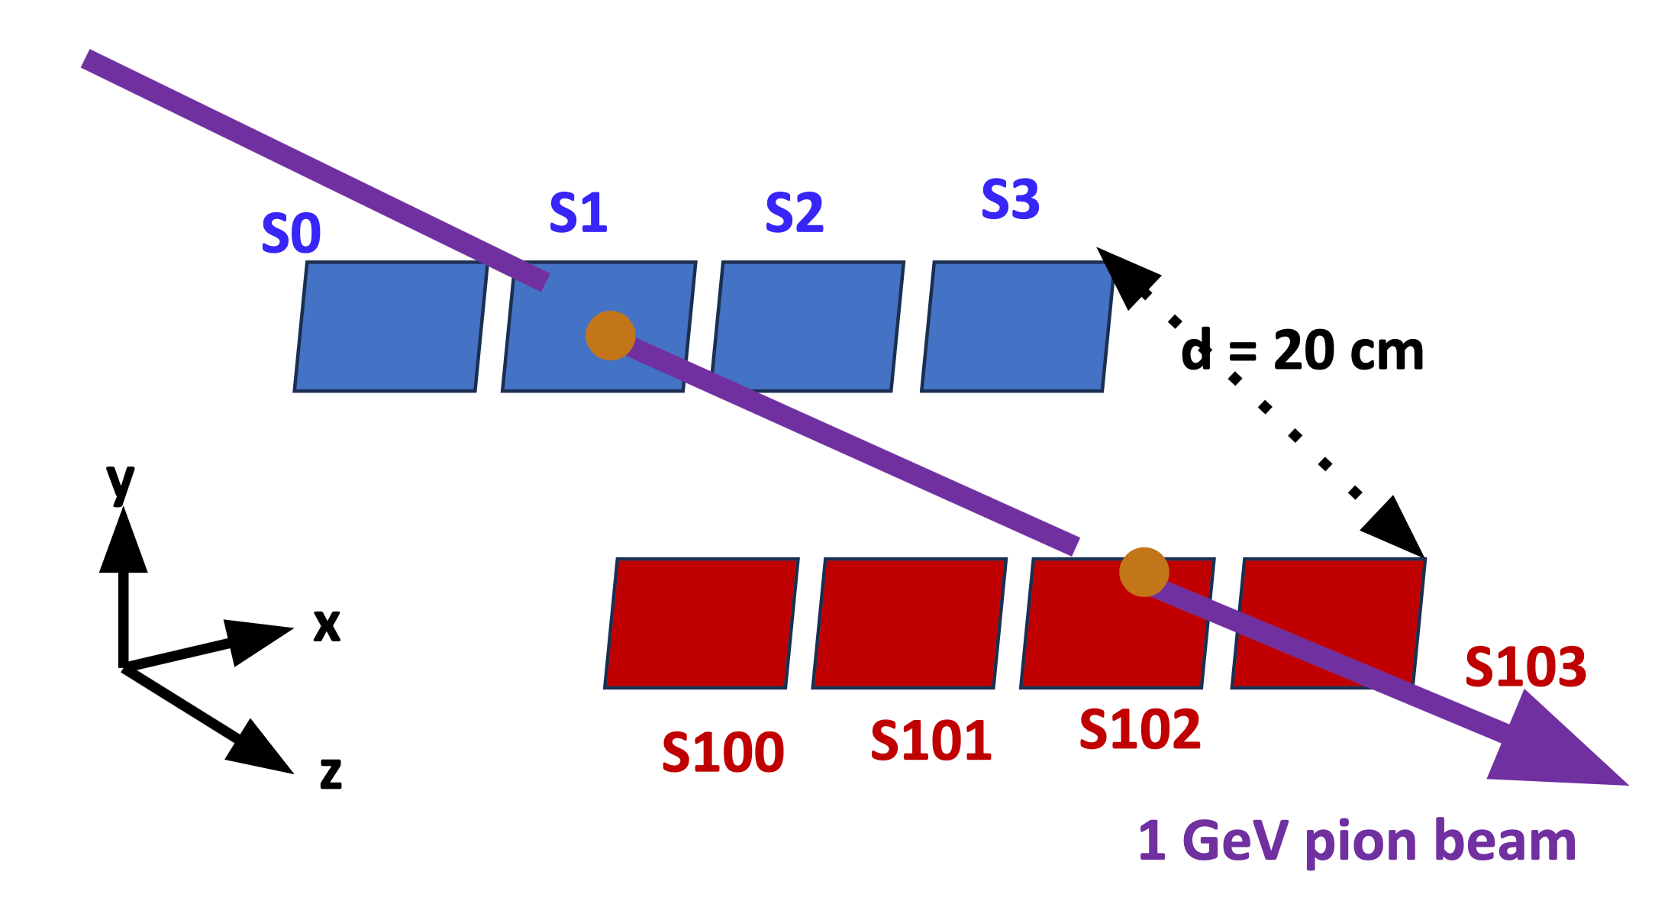
\includegraphics[width=0.9\linewidth]{Figures/geom.png}
    \caption{Telescope geometry and setup in simulation.}
    \label{fig:simgeom}
\end{figure}

The telescope is modelled in GEANT4 as a quad module of four identical
MALTA2 sensors placed in series along the beam axis. Each sensor is a
$1.8\times0.9~cm^2$ monolithic CMOS pixel matrix with a
pixel pitch of \SI{36.4}{\micro\meter}, giving a $512\times224$ pixel grid.
The sensors are separated by a fixed spacing, so a particle crosses the
planes sequentially. Small time offsets between planes, arising from their
relative position and readout propagation, are applied per sensor.

Primaries are generated per event with a configurable multiplicity. The
first primary in each event is the signal (a \SI{1}{\GeV} $\pi^{+}$)
incident perpendicular to the sensor plane; any additional primaries are
background (\SI{10}{\MeV} $e^{-}$). Each primary is placed at a random
position within the active area and assigned a global time
$t = N_\text{evt}\,t_\text{veto} + \delta t$, where $N_\text{evt}$ is the
event index and $\delta t$ is a random intra-spill offset up to
\SI{2}{\micro\second}. Signal and background therefore overlap in time and
are distinguished only by their truth label, not by arrival time.

Energy deposition in each sensor is digitized with the parametric MALTA2
response (charge collection, threshold, and timing), and the resulting
pixel hits are reconstructed per plane. Truth provenance
(event ID and track ID) is propagated through digitization to allow exact
signal-to-hit association for the efficiency and tracking studies that
follow.

\subsection{Time Resolution (no background)}
\textcolor{red}{Plot: Time resolution (compare: without background, with 1,2,3 particles per event)}
Validated with data.

\subsection{Background rate}
Explain the expected background at the location of the FMT (from Amelia's plots?):
\begin{itemize}
    \item Select region of $1\times\SI{2}{\square\centi\meter}$ with highest hit rate.
    \item Show distribution of hits per $\SI{2}{\micro\second}$ event
    \item Show PDG code of background particles. Is it primarily photons and electrons/ positrons?
\end{itemize}

Explain the simplifications/ assumptions that go into the MALTA2 simulation.
\begin{itemize}
    \item Identify maximum expected background hit rate per sampled event.
    \item Spatial distribution is approximately flat within individual MALTA2 sensor.
\end{itemize}

\subsection{Hit efficiency with background}
\textcolor{red}{Plot: Hit efficiency of a signal particle versus background rate per event:}
\begin{itemize}
    \item Position of background and signal is random in MALTA2 sensor.
    \item Keep time window of background particles within \SI{10.2}{\nano\second}.
    \item Increase number of background particles that fall within this. (Expectation from Lucian: Efficiency is still >90\% for 1,2,3 background particles but decreases drastically for >3 particles.
\end{itemize}



\subsection{Tracking efficiency, potential spatial/temporal resolution with background}
This subsection can target the proper tracking efficiency using 2 FMT planes.
\begin{itemize}
    \item Obtain hits per plane.
    \item Reconstruct a track from the two planes.
    \item Calculate pointing resolution of the track. In the simulation, signal is incident perpendicular onto the sensor. How is the direction reconstructed from the track?
\end{itemize}

\subsection{Matching capability with background}